\section{Chapter Overview}
The first step in creating \iac{FPGA} based network of \acfp{ADPLL} is the design of the \ac{ADPLL} itself, which will be addressed in this chapter. The nature of \iac{FPGA} necessitates compromises in the design of a certain blocks, limiting direct transfer from \ac{ASIC} designs. In this chapter the potential designs for each individual block, or module, investigated will be explained and the case for their selection in \iac{FPGA} based \ac{ADPLL} made. A number of blocks have implemented by purely digital circuitry and as such can be transferred in their entirety from \iac{FPGA} and vice versa. However, those that will be used to emulate mixed-signal circuitry, such as the \ac{DCO} and \ac{PFD}, will be examined in greater detail. \Iac{RTL} diagram of the \ac{ADPLL} topology that will be used in the following sections is shown in Figure \ref{fig:network_adpll}.
\begin{figure}[h]
	\centering
	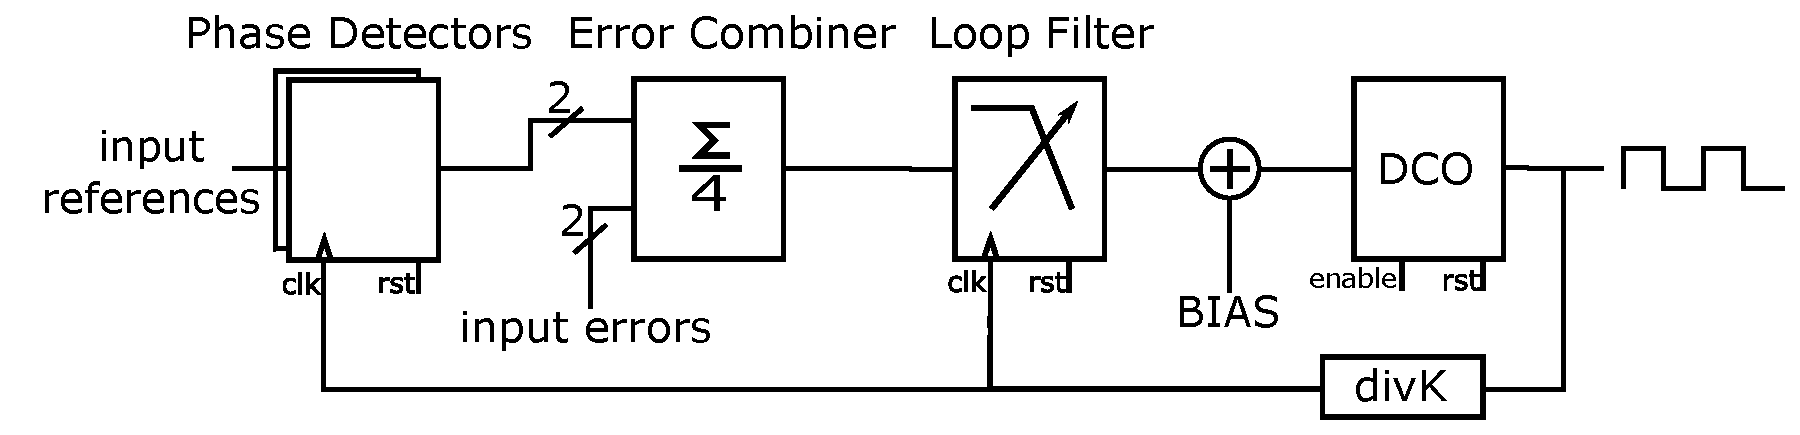
\includegraphics[width=\textwidth]{../network_adpll}
	\caption{\acs{ADPLL} designed for use in a Cartesian grid network.}
	\label{fig:network_adpll}
\end{figure}

It is Important to note that despite a Cartesian grid leading to four neighbours, only two phase detectors are required per oscillator. Borrowing matrix indexing, and choosing the oscillator located at index $(i,j)$, $i,j \neq 1,N$ where $N$ is the number of oscillators in each direction, comparison need only be done with the signals generated by oscillators located at $(i-1,j)$ and $(i,j-1)$. The comparison with oscillators $(i+1,j)$ and $(i,j+1$) will be carried out in those \acp{ADPLL}, and the negation of the errors measured, used in the \ac{ADPLL} located at $(i,j)$.

\section{Digitally Controlled Oscillators}
The choices made in the design of the \ac{DCO} have the greatest impact on the effectiveness of the overall platform and which use cases the \ac{ADPLL} is suitable for, as all performance benchmarks are done using the waveform this block generates. This project will address three distinct designs of \acp{DCO} suitable for implementation on an FPGA, two derived from the clocks generated by the \acp{FPGA} own distribution network and one generated independently of this clock, using a chain of inverters. These are not the only ways in which an oscillator could be synthesised on \iac{FPGA}, however, other designs were deemed to be unsuitable for extensible and portable implementations.
%TODO delete if space needed
A prime example of this, is the use of Xilinx proprietary \texttt{IODELAY} blocks to create an oscillator, as detailed in Xilinx Application Note XAPP872 \cite{iodelay}. The key idea here is that the bulk of the period is made up by the propagation time through one of the \texttt{IODELAY} blocks, which can be set at implementation time. This is combined with a section of an inverter chain, and a multiplexer is used modify the length of this segment, the output of which is fed back into the \texttt{IODELAY} block. This method was discarded as the number of \texttt{IODELAY} blocks is very limited, so expanding to a larger network would be impossible, and as they are all located around the edge of the chip, not suited to the construction of a Cartesian grid.
%TODO delete if space needed

The main issue with the creation of \acp{DCO} on \iac{FPGA}, is the inability to create mixed-signal circuits, such as those used on \iac{ASIC}. Therefore the \ac{FPGA} based oscillator must emulate the behaviour of a mixed-signal circuit in some way.

\subsection{\acs{FPGA} Driven, Linear Period \acs{DCO}}
\begin{figure}[h]
	\centering
	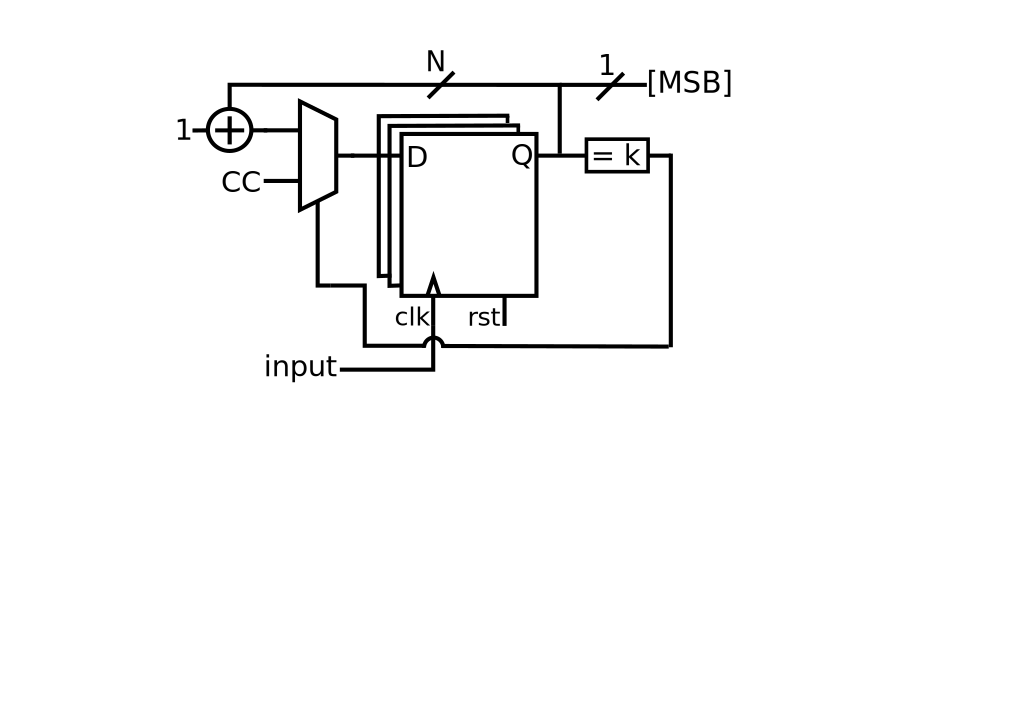
\includegraphics[width=0.6\textwidth]{../osc1}
	\caption{\acs{FPGA} driven, linear period \acs{DCO} \ac{RTL} Diagram.}
	\label{fig:osc1}
\end{figure}
The first design of \ac{DCO} to be examined, is of the type used by Zianbetov in his \ac{ADPLL} network test bed and relies on a counter driven by the clock manager on the \ac{FPGA} \cite{zianbetov2013phd}. At each event on the \ac{FPGA} provided clock, a counter is incremented, overflowing upon increment past the maximum possible value. The \ac{MSB} of this counter forms the waveform generated by this oscillator, the period of which is controlled through an adjustable value that is loaded into the counter once overflow is reached, and forms the starting point for the counter. The period of oscillation is given by:
\begin{equation}
	T_{osc} = \big(2^{width} -~(BIAS+CC)~\big)\times T_{FPGA}
\end{equation}
where $T_{FPGA}$ is the clock period of the \ac{FPGA}, $CC$ is the control code input, $BIAS$ centres the oscillator in the middle of the tuning range in the event that the control code is zero and $width$ is the width of the counter used. As the only variable here is the control code, the period step of this design is $T_{FPGA}$, thereby providing period linearity with respect to the control code. This is the key advantage of this design, as most \ac{ASIC} implementations of \iac{DCO} are also linear in period. The other main reason to choose this design, is that its \ac{FPGA} clocked nature allows for exact control over the frequency of operation, and the number of tunable parameters make it possible to configure multiple ways to achieve the same frequencies of operation. Combined, these attributes make it very easy to create an oscillator that emulates the behaviour of a design intended for \iac{ASIC}, however, at a greatly reduced frequency. This restriction on the frequency of operation arises out of the period step size, which in order to obtain a good resolution must be orders of magnitude smaller than the intended period. As the output waveform is taken from the counter's \ac{MSB}, the reload value of the counter must never go beyond $2^{width-1}$, as otherwise the output waveform will become a constant 1. As the reload value varies the low time of the \ac{MSB}, if the desired output waveform is a square wave, this design will not be suitable.

Being \ac{FPGA} clocked this design has pseudo-deterministic characteristics, with each period step being almost identical across oscillators and over the entire tuning range, unlike \iac{ASIC} where process variation will impact the layout of a high frequency oscillator. The only variation in this design will come, ironically, from jitter or skew in the \ac{FPGA}'s clock distribution network, which as the frequencies will be in the hundreds of MHz is very minor. In the case of the Xilinx \acl*{Nexys} this is at most 100 picoseconds, or 0.05\% of the period of an intended output clock at 5 MHz. To put this value into perspective, on this board the minimum value of $T_{FPGA}$ that could be used to drive this oscillator is $3.875~\si{\nano\second}$, $1.935\%$ of the period.

The resulting \ac{DCO} is best suited to applications that do not seek to gain a better understanding of oscillator performance, but rather those focused on validating the entirely digital blocks in the system, the role in which Zianbetov and Shan used this type of oscillator \cite{zianbetov2013phd,shan2014phd}.

\subsection{\acs{FPGA} Driven, Linear Frequency \acs{DCO}}
\begin{figure}[h]
	\centering
	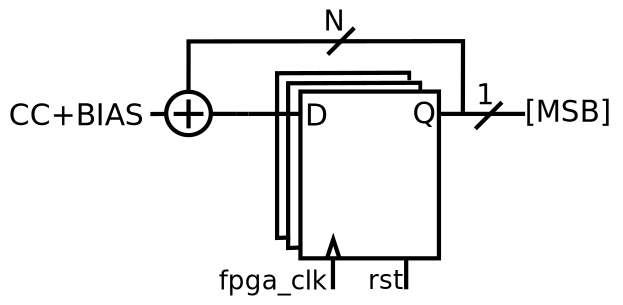
\includegraphics[width=0.6\textwidth]{../osc2}
	\caption{\acs{FPGA} driven, linear frequency \acs{DCO} \ac{RTL} Diagram.}
	\label{fig:osc2}
\end{figure}
The second \ac{FPGA} clocked oscillator is similar in most attributes to the above design but eschews period linearity for frequency linearity. Again the overflow property of a counter is used with the counter's \ac{MSB} as the block's output, however, this time it forms a square wave. Rather than setting the reload value of the counter, instead the increment is adjusted depending on the control code, thus requiring $\frac{2^N}{BIAS+CC}$ increments to overflow. Accordingly the frequency of operation is set by:
\begin{equation}
	f_{osc} = f_{FPGA}\times\frac{BIAS+CC}{2^{width}}
\end{equation}
Here the control code $CC$ and $BIAS$ are added to the value stored in the accumulator at each event of the \ac{FPGA} clock, until overflow is reached. This occurs at $2^{width}$ where, as before, $width$ is the bit width of the counter, thus valuing each control code increment at $\frac{f_{FPGA}}{2^{width}}$ Hz. As with the previous design, this oscillator is better suited to frequencies where the output of the \ac{DCO} is orders of magnitude lower than the clock signal driving it, as this ensures that the incremental change due to the control code remains a small fraction of the period.

This design is just as configurable as its linear-in-period counterpart, and well suited to the low frequency emulation of \ac{ASIC} based oscillators that are themselves linear in frequency. In sharing the \ac{FPGA} as a clock source, the pseudo-deterministic characteristics return, once more meaning this oscillator is better used for testing, simulating or verifying other blocks in the system.

\subsection{Ring Oscillator}
The best approximation of the non-idealities of \iac{ASIC} \ac{DCO} implementation can be obtained using \iac{RO}, also known as an inverter ring, as the \ac{DCO}. In \iac{ASIC} \iac{RO} is constructed by connecting a number of inverters back in a chain, with the output of the last NOT gate fed into the input of the first. As true inverters are not available on \iac{FPGA}, they are replaced by inverter primitives, constructed from look-up tables. The inverter ring is an inherently unstable circuit, that leverages the propagation delay through an odd number of inverters to create a waveform that, when viewed at a fixed position, is a square wave. 
\begin{figure}[h]
	\centering
	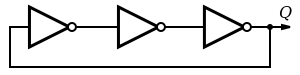
\includegraphics[width=0.4\textwidth]{../RO-wiki}
	\caption[Basic ring oscillator \ac{RTL} diagram]{Basic ring oscillator \ac{RTL} diagram \cite{ro_wiki}.}
	\label{fig:ro_wiki}
\end{figure}

The output value of the inverter at the end of the chain changes a non-zero amount of time after the input to the first element is set. It can be trivially shown that if the number of inverters is odd, this will be the inverse of the value initially applied to the first element. This sets in motion an oscillation, the period of which is governed by the number of inverters in the chain. The formula to calculate the oscillator's period is simple:
\begin{equation}
	T_{osc} = 2\times \tau_{inv} \times N
\end{equation}
Here, $\tau_{inv}$ is the propagation time through one inverter, $N$ is the number of inverters in the chain and the multiple of two arises from the necessity to invert twice to produce a square wave.

The main advantage of this type of oscillator stems from its similarity to that used on \iac{ASIC} which leads to many non-idealities carrying over from the truly mixed-signal implementation. Rather than being just a tool used to validate other modules, the performance of this oscillator can be analysed more deeply as well as the performance of networks containing it. Koskin \textit{et al} tested theories proposed regarding the synchronisation of oscillators during his PhD using this type of oscillator implemented on \iac{FPGA} \cite{koskin2019phd,theboys2019}. Also in this design's favour is the period step size, four times the inverter propagation delay, which was found experimentally to be within in the region of a nanosecond on Xilinx Artix-7 and Zynq \acp{FPGA}.

While it is advantageous for the purposes of analysis that this design is affected by variation in temperature, implementation and other non-idealities, this brings with it challenges not present in a true mixed-signal design. In a design intended for \iac{ASIC}, the designer has near total control over the placement of circuit elements, however, the \ac{FPGA} based counterpart control the designer may only set the region within the oscillator will lie, and the \acs{EDA} tool is responsible for the exact placement. Unlike the \ac{ASIC} implementation, in which the propagation delay through each element of the ring is well bounded, the lack of control over placement means that the propagation time through each inverter is not well bounded and may vary wildly. This makes it time consuming to ensure that the frequency tuning ranges of each oscillator match that desired, and making use of this oscillator less straight-forward than that of the previous two designs. This is compounded by the simulation tools in the \ac{EDA} packages intended for \acp{FPGA} being unable to accurately simulate the time delays, thus negating any benefit of test benches for the alignment process.

\section{Frequency Divider}
Many \aclp{PLL} (\acsp{PLL}), be they digital or analogue, incorporate a frequency divider in the feedback path, so that comparisons can be made with a reference operating at a lower frequency. This is a feature that is advantageous for \ac{ADPLL} networks, as comparisons using this divided clock allows the synchronisation signal sent between modules to be of a frequency orders of magnitude lower than that of the clock distribution network, and thus requiring circuitry that consumes significantly less energy. This division can be obtained trivially on \iac{FPGA} by a number of means; of which this thesis will mention just two. The first of these methods allows for integer division, by inverting a signal each time a counter reaches a certain value, $k$. When this condition is true the value stored in the counter is also reset to zero, thus dividing the generated clock frequency by $2k$.
\begin{figure}[h]%
	\centering
	\subfloat[Divider 1]{{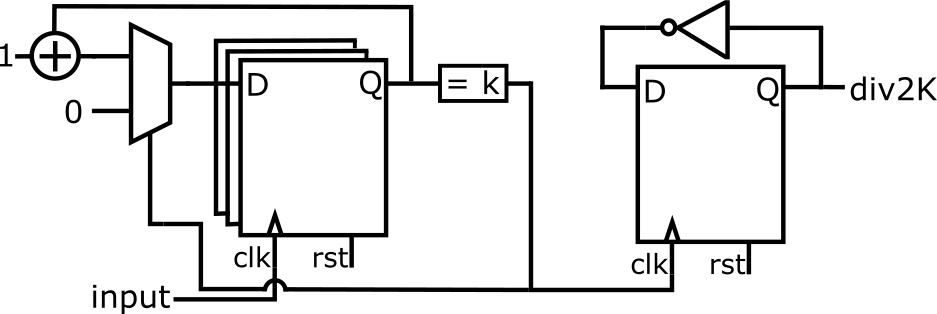
\includegraphics[width=0.6\textwidth]{../divider1} }}\\
	\subfloat[Divider 2]{{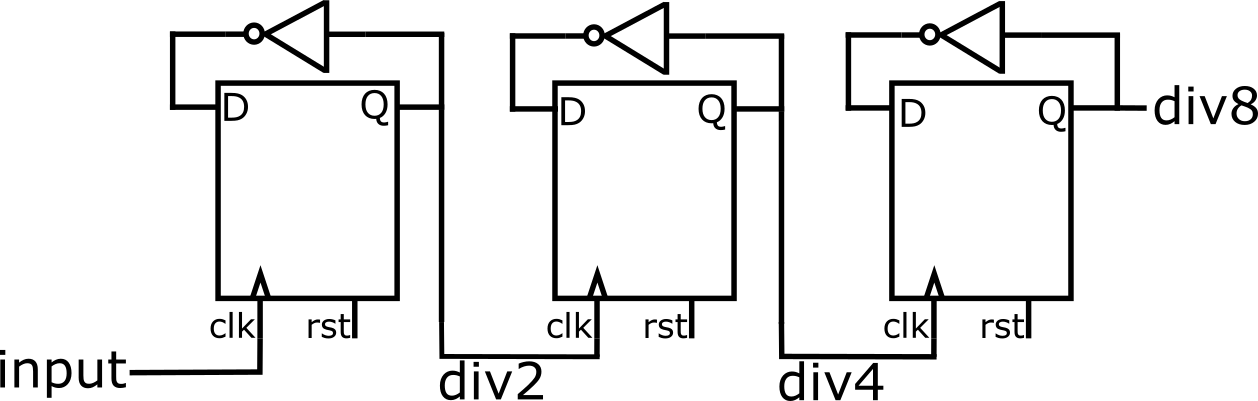
\includegraphics[width=0.6\textwidth]{../divider2} }}%
	\caption[Frequency divider \ac{RTL} diagrams]{Frequency divider \ac{RTL} diagrams.}
	\label{fig:divs}
\end{figure}

By limiting division to powers of two, the second option ca simplify the divider by the removal of any comparison logic. One flip-flop and an inverter are required per power of two. As in Figure \ref{fig:divs} (b), the inverted $\overline{Q}$ output of each flip-flop is inverted and connected to the $D$ input, with the non-inverted $Q$ of the previous flip-flop acting as the clock. The first flip-flop in the chain is clocked by the \ac{DCO} output. 

\section{Phase Detector}
Three potential \acl{PD} designs will be addressed in this thesis, sign-only detection with a Bang-Bang Detector, \ac{FPGA} clocked detection using \iac{FSM} and an emulation of \iac{TDL} using inverter primitives to create a delay, similarly to the \ac{RO} seen previously. All designs will have to have a representation for both situations where the generated signal leads and lags the reference signal, and for the magnitude of this difference. Both can be combined using a signed binary representation of the difference, such as two's complement. Two's complement is easily implemented, as operations can be carried out by the same hardware as unsigned arithmetic. The sign convention for phase error assigns the positive values to the situation where the generated signal lags the reference, and vice versa for the leading case. Apart from the Bang-Bang Detector, each design features two blocks, one to determine the sign of the error and a second to estimate the magnitude. These blocks could theoretically be mixed-and-matched, but as they operate on different paradigms, no benefit would be obtained.

\subsection{Bang-Bang Detector}
A Bang-Bang Detector is a sign-only detector, thus outputting a phase error a single bit wide. This can be accomplished using a single flip-flop, with the reference signal acting as the clock, in this case using the rising edge, a design verified by Predraig in his 2011 thesis \cite{predraig}. The generated signal is applied to the $D$ input, thus when a rising edge is seen on the reference, the value of the generated signal is held as the $Q$ output until the next rising edge of the reference. If the generated signal has gone high prior to the reference, and leading it, the value of $Q$ will be 1, thereby matching the expected sign behaviour. Trivially it can be seen that the case where the generated signal lags the reference the $Q$ will show $0$.
\begin{figure}[h]
	\centering
	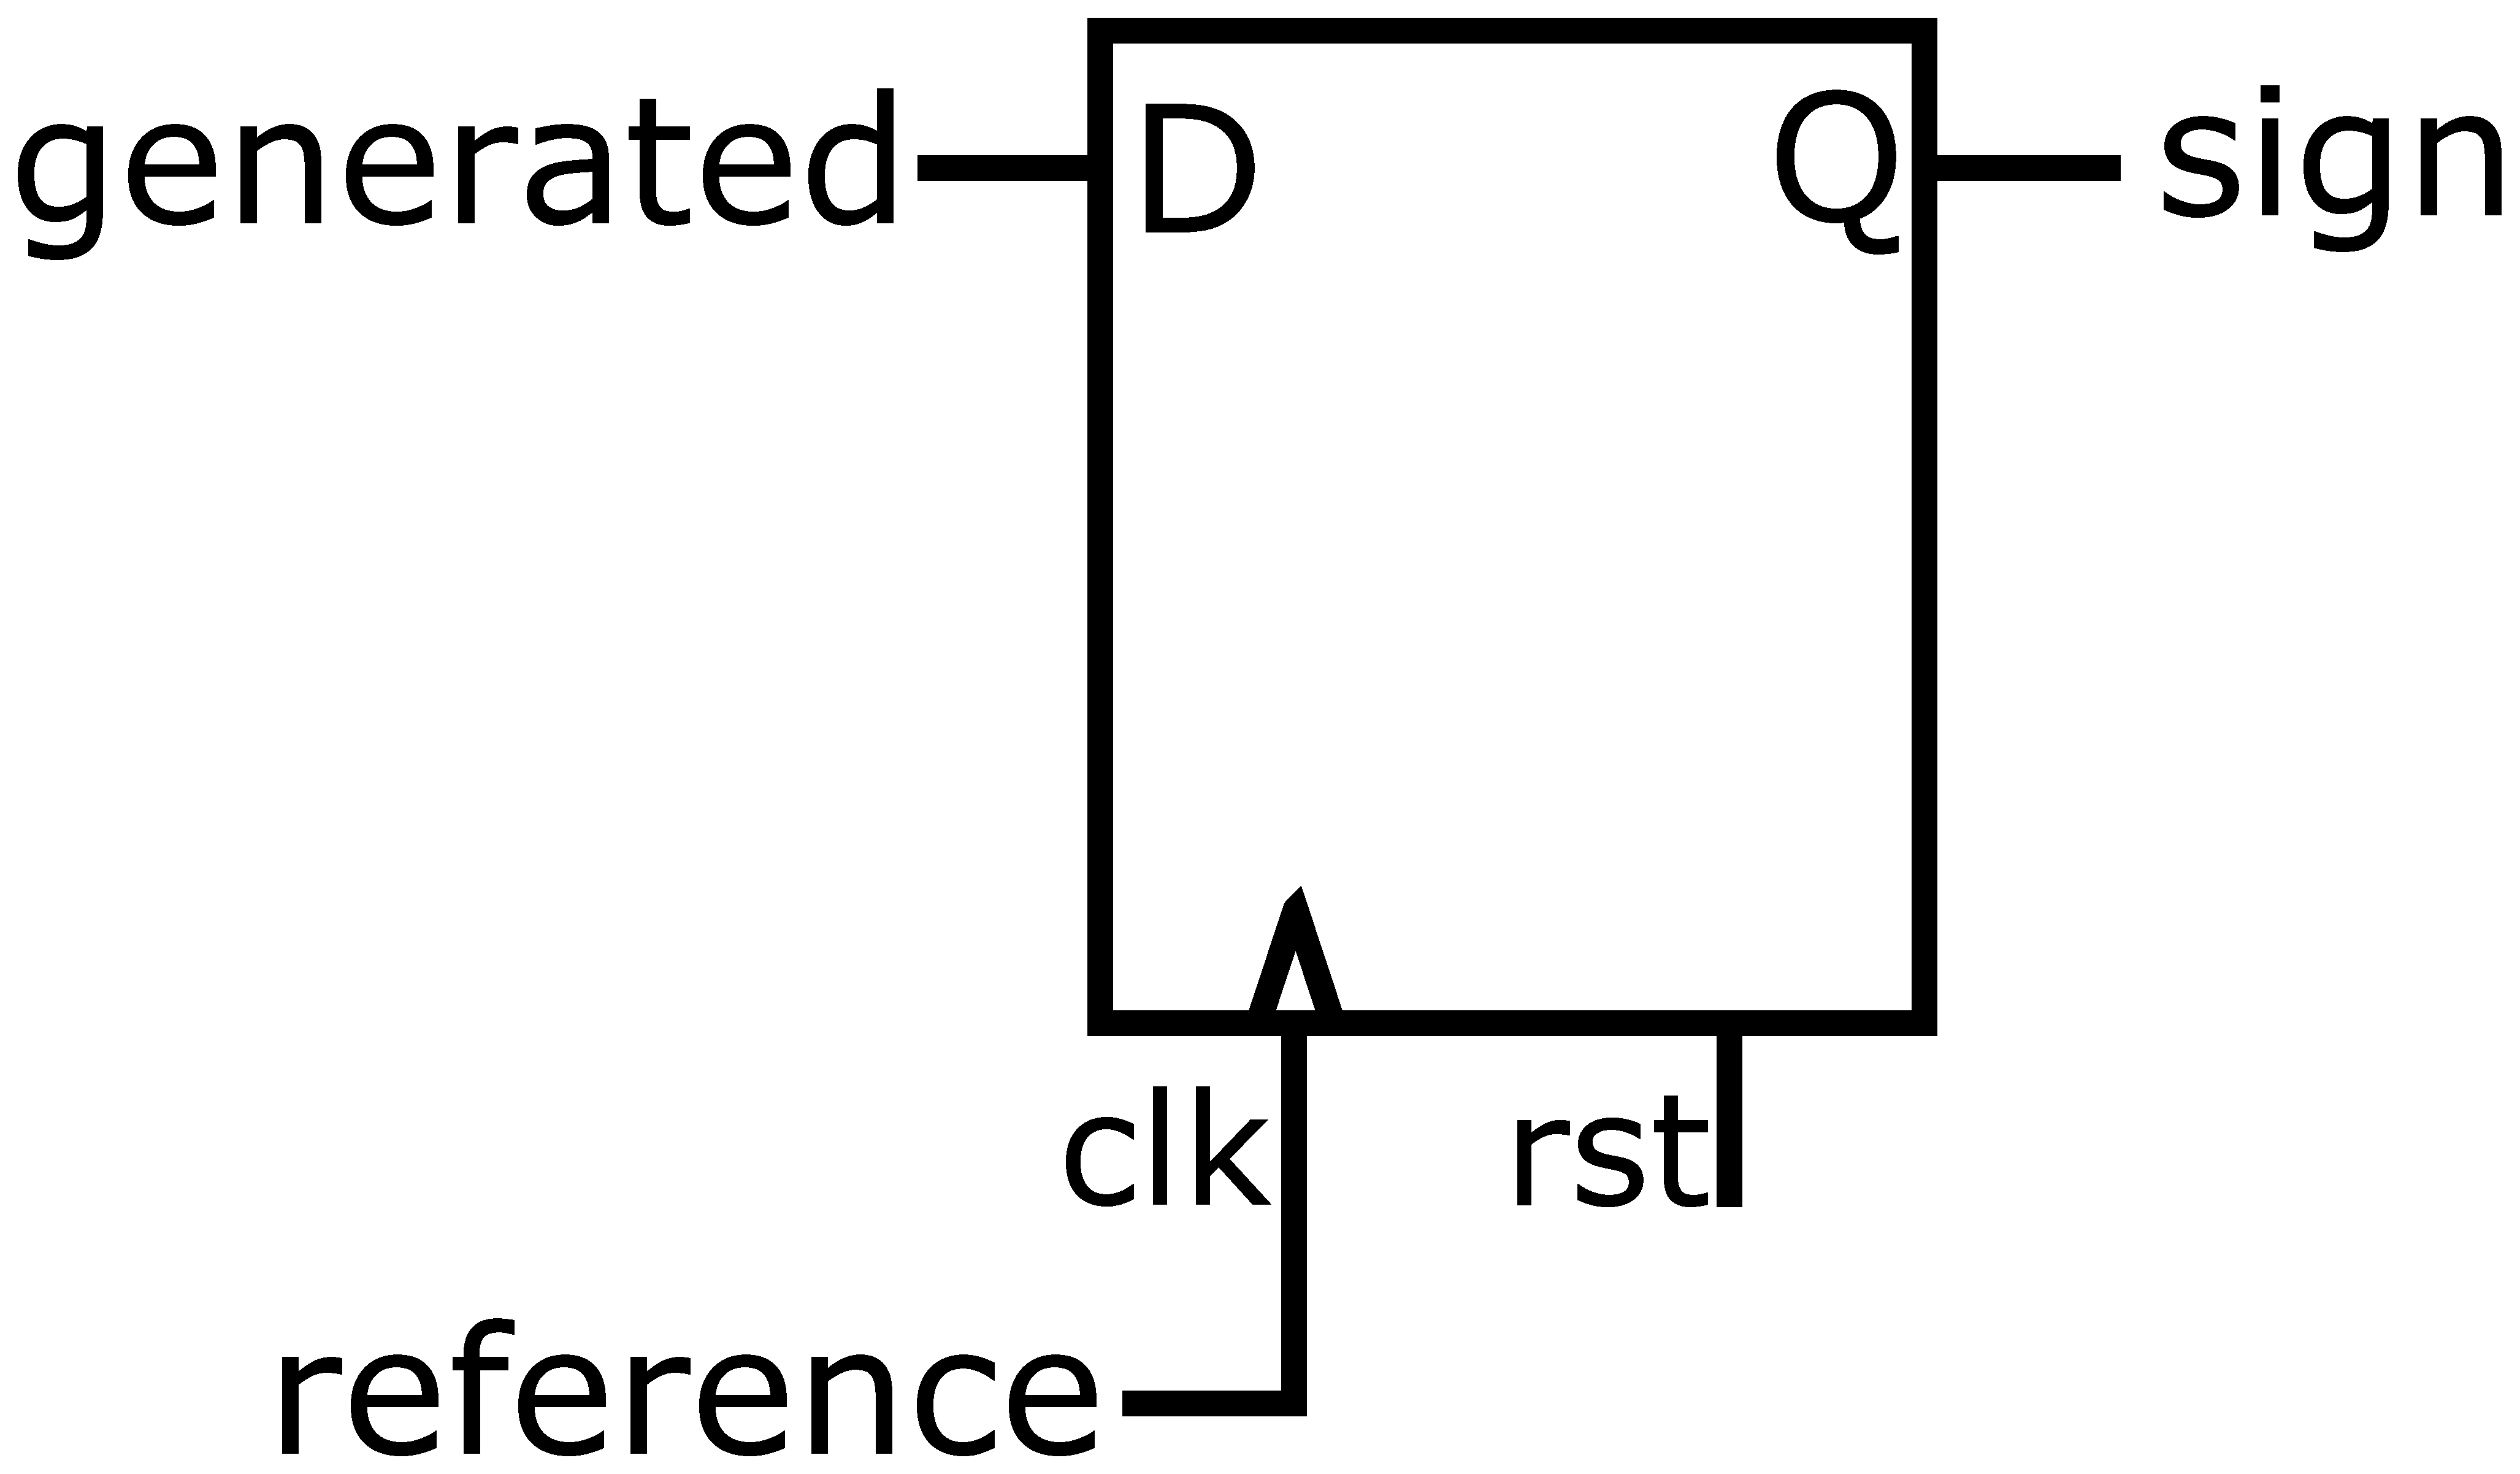
\includegraphics[width=0.4\textwidth]{../BB}
	\caption[Bang-bang phase detector \ac{RTL} diagram]{Bang-bang phase detector \ac{RTL} diagram.}
	\label{fig:bang_bang}
\end{figure}

This design is simple but effective, and can be used without a loop filter, albeit with a very limited oscillator tuning range. This is an especially valuable attribute at early stages of platform development, as it may be used in order to test that other aspects of the system work as intended. The binary resolution of this detector, however, restricts its usefulness ,as the \ac{ADPLL} cannot react more quickly to larger phase differences.

\subsection{\acs{FPGA} Clocked Phase Detector}
The easier to implement of the two designs, uses a combination of a state machine to determine which edge occurred first, and to control a two's complement up-down counter, which acts as the \ac{TDC} in this detector, and estimates the magnitude of the error.

\subsubsection{State Machine Based Detection}
While sign detection clocked by the \ac{FPGA} can be performed in a variety of ways, a state machine is a straightforward way in which to accomplish this. \Iacl{FSM} consists of three main components: the states themselves, the next state logic and the output logic. In this case the next state logic is the generated and reference signals, and the output logic sets the count instructions for the up-down counter, as well as ensuring the phase error output is held constant between measurement periods. The \ac{FSM} will have a state representing the case where either the reference or generated signals occurred first, in addition to a wait state used between the end of one measurement interval and the commencement of the next. Two types of \ac{FSM} exist, Moore and Mealy Machines, the difference being that Moore Machines base their output only on the current state, while Mealy Machines do so on both the current state and the inputs to the system. If a Moore Machines is used an extra state is required in order to hold the value of the phase error at the end of the measurement interval.

As this design is clocked by the \ac{FPGA}, the phase error is quantised to the the \ac{FPGA} clock periods, thus setting the resolution of the design. While, depending on the oscillator design, the generated clock may be synchronous to the \ac{FPGA}, the reference signal arrives from off-chip and thus will not be synchronised to the measurement clock. In order to avoid any metastability events arising from an input signal changing within the set-up and hold times of the registers sampling them, synchroniser circuits are used to ensure the value sampled is either logic high or low at the instance of the measurement. As these synchronisers are the first \ac{FPGA} clocked elements in the measurement chain, they also act as the system's quantisers. There is no degradation in detection resolution, as the signals would be quantised to the \ac{FPGA} clock anyway.

There are three situations that may occur while the \ac{FSM} is in the waiting state. Firstly, the case where the reference signal sees a rising edge before the generated clock, and thus the generated clock is said to be lagging the reference. As previously mentioned, the convention dictates that the phase difference have a positive sign, so the counter is incremented to count in the positive direction. Secondly, if the generated signal is leading the reference, the sign of the error is negative and thus the counter is instructed to count downwards. The third potential scenario occurs when both clock signals have a rising edge within the same period of the \ac{FPGA} clock, which due to quantisation will be interpreted as both signals occurring at exactly the same time. In this case the counter receives no instruction and a zero value is stored until the next measurement interval. Once the \ac{FSM} is in a measurement state, and the counter either incrementing or decrementing, a rising edge occurring on the opposite signal to that which initiated the measurement, will end the interval.
\begin{figure}[h]
	\centering
	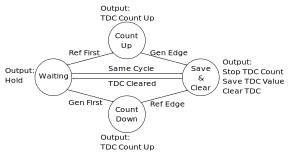
\includegraphics[width=0.8\textwidth]{../state_trans_new}
	\caption[Example State Transition Diagram for a Moore Machine]{Example State Transition Diagram for a Moore Machine.}
	\label{fig:state_trans}
\end{figure}

\subsubsection{Up-Down Counter}
The up-down counter in this design estimates the magnitude of the phase difference between the reference and generated signals. The state machine provides control instructions, indicating whether the count should be in the increasing or decreasing directions, and holds the counter in reset once the measurement interval has been completed. The counter counts in two's complement, so counting in the downward direction can be carried out by adding on the representation of -1, the binary signal containing all 1s. The other advantage of counting in two's complement is that count value is already in the correct format for the follow block, the phase detector in a regular \ac{ADPLL} or the error combiner in this instance, therefore the count value at the end of the measurement interval can be stored in a register, which maintains the output value of the phase detector between measurements. Two's complement is an advantageous way to represent signed numbers in hardware as the mathematical operations are identical to their unsigned counterparts, thus allowing use of any adder or carry hardware that may be present on the \ac{FPGA}. An important attribute of this counter is the ability to freeze the count at the minimum and maximum count values, in order to avoid a situation where the counter overflows. At high phase offsets this may cause alternation between positive and negative differences, restricting the locking range of the \ac{ADPLL}. Disallowing overflow also aligns the behaviour of this phase detector with that of those implementing delay lines, allowing better interchangeability and comparison, which for a testing platform is valuable.

This counter is best suited for use with the aforementioned \ac{FSM} sign detection circuitry, and would see no benefit from a combination with the un-clocked sign detection circuit that will be presented in the following section. This is the case as if quantisation to the \ac{FPGA} clock had not already occurred in the sign detection circuit it would occur in this counter, as increments are only possible at \ac{FPGA} clocking events, thereby enforcing quantisation to the \ac{FPGA} clock. The coarseness of this measurement, restricted to time delay increments equal to the \ac{FPGA} clock period means that it is an ideal detection method for the clocked oscillators, as the minimum phase difference that can be detected matches exactly with the minimum step by which the oscillator period can be tuned. This design can, however, be used with the \acl{RO}, provided the \acl{LF} gains are adjusted to maintain the oscillator to detector step relationship.

\subsection{SigNum Detector}\label{section:signum}
The SigNum detector is based on the methodology used in the Bang-Bang \acl{PD} seen previously, but rather than just performing sign detection, the magnitude of the phase difference can also be measured. In the case of the \ac{FPGA} clocked design, the counter handled the representation of both sign and magnitude, but as the name SigNum (Sign Number) suggests, both are handled separately in this design. The modified Bang-Bang detector establishes which signal occurred first and generates a control signal that is analogous to the time delay between a rising edge on each input signal. \Iacf{TDL} then uses this control signal to convert the phase difference between the signals to a digital signal. The magnitude is combined with the sign detected by the bang-Bang detector to form a two's complement error signal.

This method of phase detection is advantageous, as similarly to the \acl{RO}, the \ac{TDL} can be implemented using inverters, and therefore is not synchronised to the \ac{FPGA} clock. The propagation time through inverters once more sets the resolution, thus allowing a smaller step than that of the clocked designs. The disadvantages, however, are also consistent with the \ac{RO} in that the propagation time will vary significantly depending on the \ac{EDA}'s placement of the circuit. This is not as severe a limitation for the \ac{TDL} as the \ac{RO} as, while the tuning range is affected by this variation, it cannot cause the centre point to vary, whereas the impact of placement on the \ac{RO} caused both variation in range and centre frequency.


\subsubsection{Sign Detection}
The Bang-Bang detector structure changes significantly in order to provide the control signals required for the \ac{TDC}. The \ac{TDC} expects a long pulse of logic high for the duration of the measurement interval, going low once the interval has ended. The original single flip-flop design maintains a value between rising edges of the reference clock and could not generate the required pulse. Instead two flip-flops are used, each clocked on an input signal with their $D$ inputs connected to logic high. The $Q$ outputs of these registers are connected to \iacs{XOR} gate which generates a pulse as long as a rising edge has only been seen on one signal. Once a second rising edge occurs, the \acs{XOR} output will be set to 0, thus terminating the pulse. On completion of the measurement interval, the flip-flops must be reset in preparation for the next measurement cycle, and this can be accomplished by ANDing together the $Q$ outputs of each signal, producing a \texttt{clear} signal that will go high when both flip-flops have a logic high output.

To determine the sign itself, the clock edge which first had a rising edge must be recorded, and this can be done by setting \iac{SR} latch if the rising edge of the generated signal occurs first and resetting in the case of the reference clock having the first rising edge. Looking at the whole measurement cycle, however, it is apparent that all four combinations possible of two inputs occur, putting the \ac{SR} latch into which the output is undefined. This problem can be avoided through careful design. Examining the truth table in Table \ref{table:sr_tt}, the combination to be avoided is the presence of a 1 on both outputs, precisely the situation seen at the end of the measurement interval. In order to avoid the undefined state occurring at the end of the measurement interval, both inputs and outputs to the \ac{SR} latch can be inverted using a NOT gate. Table \ref{table:sr_tt} also illustrates how the $\overline{Q}$ output now behaves as $Q$ did previously, however, the end of measurement state where both input registers have been triggered now causes the \ac{SR} latch to enter the hold state, where it maintains the previous values. The sign, $\overline{Q}$ of the \ac{SR}, can then be loaded into a register using the \texttt{clear} signal generated previously, to maintain it until the next measurement completes.
\begin{table}[ht]
	\begin{center}
		\begin{tabular}{cc|cc}           
			$S$&$R$&$Q$&$\overline{Q}$\\
			\hline
			0&0&$Q_{n-1}$&$\overline{Q}_{n-1}$\T\\
			0&1&0&1\T\\
			1&0&1&0\T\\
			1&1&\multicolumn{2}{c}{undefined}\T\\					
		\end{tabular}
		\caption{SR latch truth table}
		\label{table:sr_tt}
	\end{center}
\end{table}

This, however, ignores the potential for metastability which may arise if both signals have a rising edge within an extremely short period of time. While it may be feasible in other systems to dismiss this occurrence as a low probability event, the goal of \iac{PLL} is to reduce the time delay between rising edges to zero. This increases the possibility of a collision occurring, which may lead to indeterminate behaviour in other parts of the feedback network. In order to avoid this in \iac{ASIC}, an arbitration circuit is placed between the \ac{SR} latch and the register storing the sign between measurements, which will default to one of the two signals in this case. This is, however, a mixed signal circuit, such as that proposed by Tierno \textit{et al} (2008) and implemented by Zianbetov and Shan \cite{tierno2008wide,zianbetov2013phd,shan2014phd}, which requires two \ac{PMOS} and two \ac{NMOS} transistors and cannot be implemented on \iac{FPGA}. As the output of the \ac{SR} latch will be indeterminate prior to the detection of the first edge, the impact of both edge detection registers' output is that the \ac{SR} latch attempts to hold this indeterminate value as an output. To avoid this unwanted behaviour the arbiter present on \iac{ASIC} is replaced by a second \ac{SR} latch, connected as in Figure \ref{fig:arbitration}. This ensures the value presented to the register storing the sign is always determinate.
\begin{table}[!ht]
	\begin{center}
		\setlength{\tabcolsep}{.5\tabcolsep}
		\begin{tabular}{l|cc|cc|c|cc|c}           
			When&$Gen$&$Ref$&$\overline{Gen}/S^a$&$\overline{Ref}/R^a$&$Q^a$&$S^b$&$R^b$&$Sign/Q^b$\\
			\hline
			Between Measurements&0&0&1&1&\multicolumn{1}{c|}{undefined}&\multicolumn{2}{c|}{01 or 10}&\multicolumn{1}{c}{0 or 1}\T\\
			Ref. First&0&1&1&0&1&0&1&0\T\\
			Gen. First&1&0&0&1&0&1&0&1\T\\	
			Measurement Complete&1&1&0&0&$Q^a_{n-1}$&$\overline{Q}^a_{n-1}$&$Q^a_{n-1}$&$\overline{Q}^a_{n-1}$\T\\					
		\end{tabular}
		\caption{Sign detector truth table}
		\label{table:sign_tt}
	\end{center}
\end{table}
\begin{figure}[h]
	\centering
	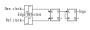
\includegraphics[width=0.8\textwidth]{../simple_sign_detection}
	\caption[Example Sign Detector]{Example Sign Detector.}
	\label{fig:arbitration}
\end{figure}

\subsubsection{Tapped Delay Line}
To complement the asynchronous sign detection circuit, an asynchronous \ac{TDC} is also required, as otherwise there would be no benefit to using the above method over the more easily understood \ac{FSM} based design, as quantisation to the clock period would happen in the \ac{TDC} rather than the sign detection circuitry. The standard method for implementing \iac{TDC} on \iac{ASIC} is through a tapped delay line, where a signal is propagated through a chain of fixed length delays, and at the end of the measurement interval whether or not the signal has propagated to each point in the chain is recorded. This architecture is illustrated in Figure \ref{fig:simple_tdc}. As with the mixed signal circuitry previously addressed, \iac{TDL} cannot be exactly replicated on \iac{FPGA}, but through the use of inverters it is possible to replace the unrealisable well bounded delays. As with the \ac{RO}, the delay though the inverters is loosely bounded, and significant variation between delays, in both individual \acp{TDL} and within the same \ac{TDL}, due to the implementation exists. This variation notwithstanding, the inverter pairs are a suitable replacement, and this method of time-to-digital conversion provides both resolution advantages and the presence of implementation based variation over a clocked design. These attributes +prove particularly beneficial when attempting to verify theoretical results.

Similarly to the sign at the output of the detection circuit, flip-flops store the value of each tap between phase error measurements. Prior to storage, the tap values must be converted to two's complement. As the signal propagates through the taps, magnitude of the phase error is determined by how many taps the signal has passed through. Conceptually, this thermometer coding is first converted to an unsigned integer before conversion to a signed quantity based on the sign of the error.
\begin{figure}[h]
	\centering
	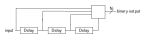
\includegraphics[width=0.8\textwidth]{../simple_tdc}
	\caption[Example \acl{TDL} Structure]{Example \acl{TDL} Structure.}
	\label{fig:simple_tdc}
\end{figure}
%TODO eugene re: why no zero output

\section{Error Combiner}
In a regular \ac{ADPLL} an error combining circuit is not required as there is never more than one reference signal, and thus the input of this block would be equivalent to the output. However in \iac{ADPLL} network, multiple reference signals are required, one for each neighbour, thus requiring combination. Simply averaging these signals was not found to be viable by Pratt and Nyugen in their original paper for analogue systems \cite{pratt1995distributed}. However, the work of Javidan \textit{et al}, showed that in a digital system this method will not result in mode locking, provided start-up is performed uni-directionally \cite{javidan2011all}.

Therefore, any intended error combiner design implementing an average, should also be reconfigurable, so that it satisfies the reconfigurability constraint. Given this is a digital system, the most straightforward way to implement this is as a weighted sum, followed by a division. The final \ac{ADPLL} network will be laid out in a Cartesian grid, so a maximum of four values will possibly be combined, with only the non-corner edge nodes having a number of neighbours that is not a power of two.
The simplest, and most processing time efficient, method of calculating the weighted sum restricts the weights to powers of two. This permits their implementation as a left bit shift, trivially achieved in hardware by a part select.
Similarly this reasoning can be expanded to the division, where the complicated division by three for a non-corner edge node is instead replaced by division by four. This means the division is implemented identically by all error combiners in the network, and implemented trivially by a right shift of two bits. Appropriate gain choice can negate the error in the averaging.

\section{Loop Filter}
The \acl{LF} in \iac{ADPLL} can be implemented as \iac{PI} controller, a circuit with many valid variations, with the exact implementation having little impact on behaviour. The first choice to be made is whether the designer wishes to implement the controller as \iac{FIR} or \ac{IIR} filter. Both methods will produce a controller that fundamentally behaves the same way, but will have a starkly different implementation. In both cases the filter can be implemented using either fractional or integer representation of the data, depending on the wishes of the designer. Carrying out computations using fractional values may be easier to understand conceptually, as the magnitude of individual paths or taps will be independent of each other, whereas using integer representations allows for a simpler hardware implementation. If fractional representation is used, it will be done with fixed-point arithmetic as the time complexity of floating point calculations is too great and the potential benefits are inconsequential. The \acl{LF} output may be applied directly to the oscillator, or an intermediate calculation done to set a bias point.

\subsection{\acs{FIR} \acl{LF}}
The \acl{FIR} implementation of the \acl{LF} will take the form presented in Figure \ref{fig:fir_pi} (a), and consists series of time delays, or ``taps'', the output of which is multiplied by a coefficient. The result of each multiplication is added together to form the filter output. Various tools, Matlab for example, can be used to compute the coefficients and number of taps required to obtain a specific filter response. Using \iac{FIR} filter is advantageous as it is always stable due to the lack of a feedback path, however a large number of taps are required to obtain a frequency response akin to that of the \ac{IIR} implementation, thus requiring an equal number of multipliers and $taps-1$ adders. Compared to \iac{IIR}, which requires just two adders, two multipliers and a flip-flop this, has a much greater hardware footprint. It is possible to condense the \ac{FIR} multiplication and addition to a single multiplier and adder, depicted in \ref{fig:fir_pi} (b), however this will take as many clock cycles to complete as there are taps. This is not viable in an \ac{ADPLL} as the filter must produce its output in a single clock cycle. In the case of any coefficient symmetry, addition can be performed prior to multiplication, thus reducing the number of multipliers for each identical coefficient.
\begin{figure}[h]
	\centering
	\subfloat[Typical FIR Filter]{{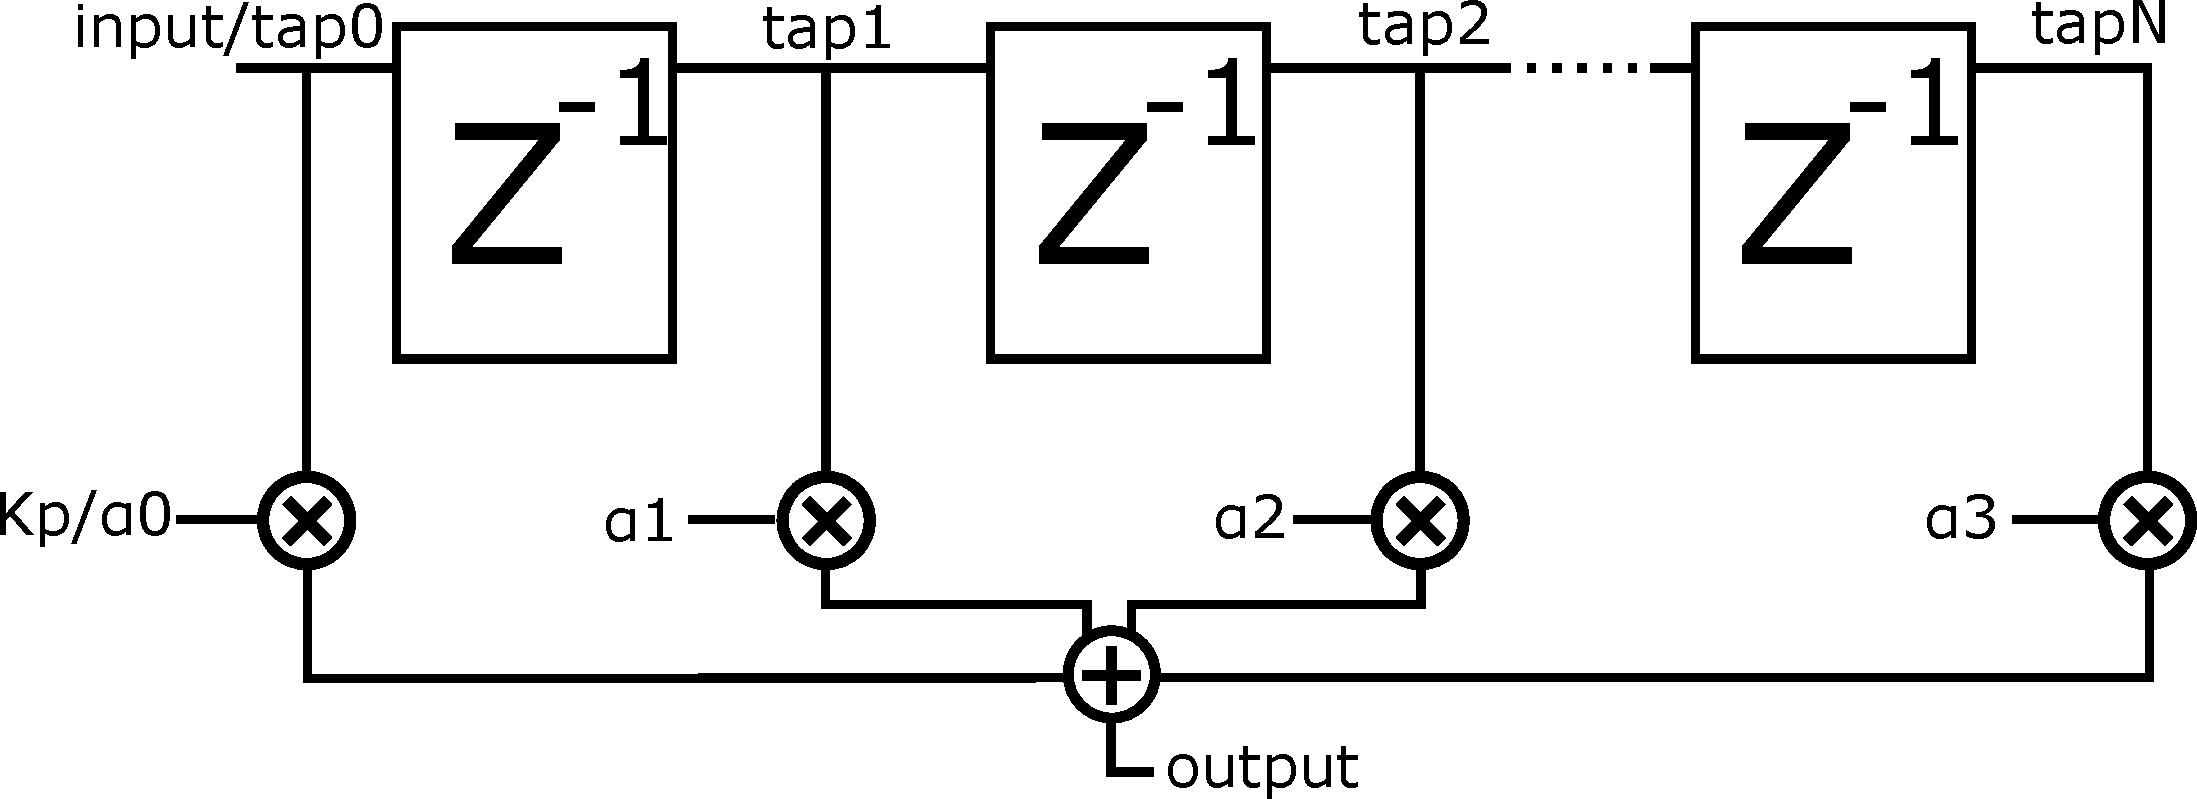
\includegraphics[width=0.6\textwidth]{../FIR_1} }}\\
	\subfloat[Single Multiplier FIR Filter]{{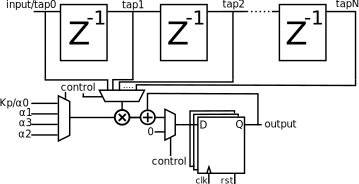
\includegraphics[width=0.6\textwidth]{../FIR_2} }}%
	\caption[\acs{FIR} \acs{PI} loop filter RTL diagrams]{\acs{FIR} \acs{PI} loop filter RTL diagrams.}
	\label{fig:fir_pi}
\end{figure}

The filter can be implemented using fixed-point arithmetic, in which the designer must ensure alignment of the radix in additions and correct radix position in multiplication results. Consequently, the fractional width of each multiplication need not be the same, most commonly used when the proportional gain, the output of the 0th tap multiplication, is significantly larger than that of the other taps. Integer arithmetic instead assumes all calculations are carried out using integers, and output of the addition stage is divided by a large number to form the module output. The integer approach simplifies the task of the designer and reduces the likelihood of incorrect calculations due to misalignment.

\subsection{\acs{IIR} \acl{LF}}
\Iac{PI} controller implemented most easily in hardware as \iacl{IIR} filter, as in Figure \ref{fig:iir_pi}. It comprises significantly fewer circuit elements than \iac{FIR} based design as the long series of taps and multipliers is not required. Instead integration is performed by a single multiplier and an accumulator. As seen before, the frequency response of the controller can be calculated using the following equation, where $\alpha$ is the proportional and $\beta$ the integral gain:
\begin{equation*}
	H(z) = \alpha + \beta\frac{1}{1-z^{-1}} = \frac{(\alpha + \beta) - \alpha z^{-1}}{1-z^{-1}}
\end{equation*}

As the scaling factor used in this multiplier is the \ac{ki} itself, reconfiguration of the integral path of the \acl{LF} can be carried out solely by varying this gain, as opposed to the \ac{FIR} solution where the value of each tap must be recalculated to change the response of the system. The combination of reconfigurability and simpler hardware, make the \ac{IIR} the more desirable \ac{LF} design.
\begin{figure}[h]
	\centering
	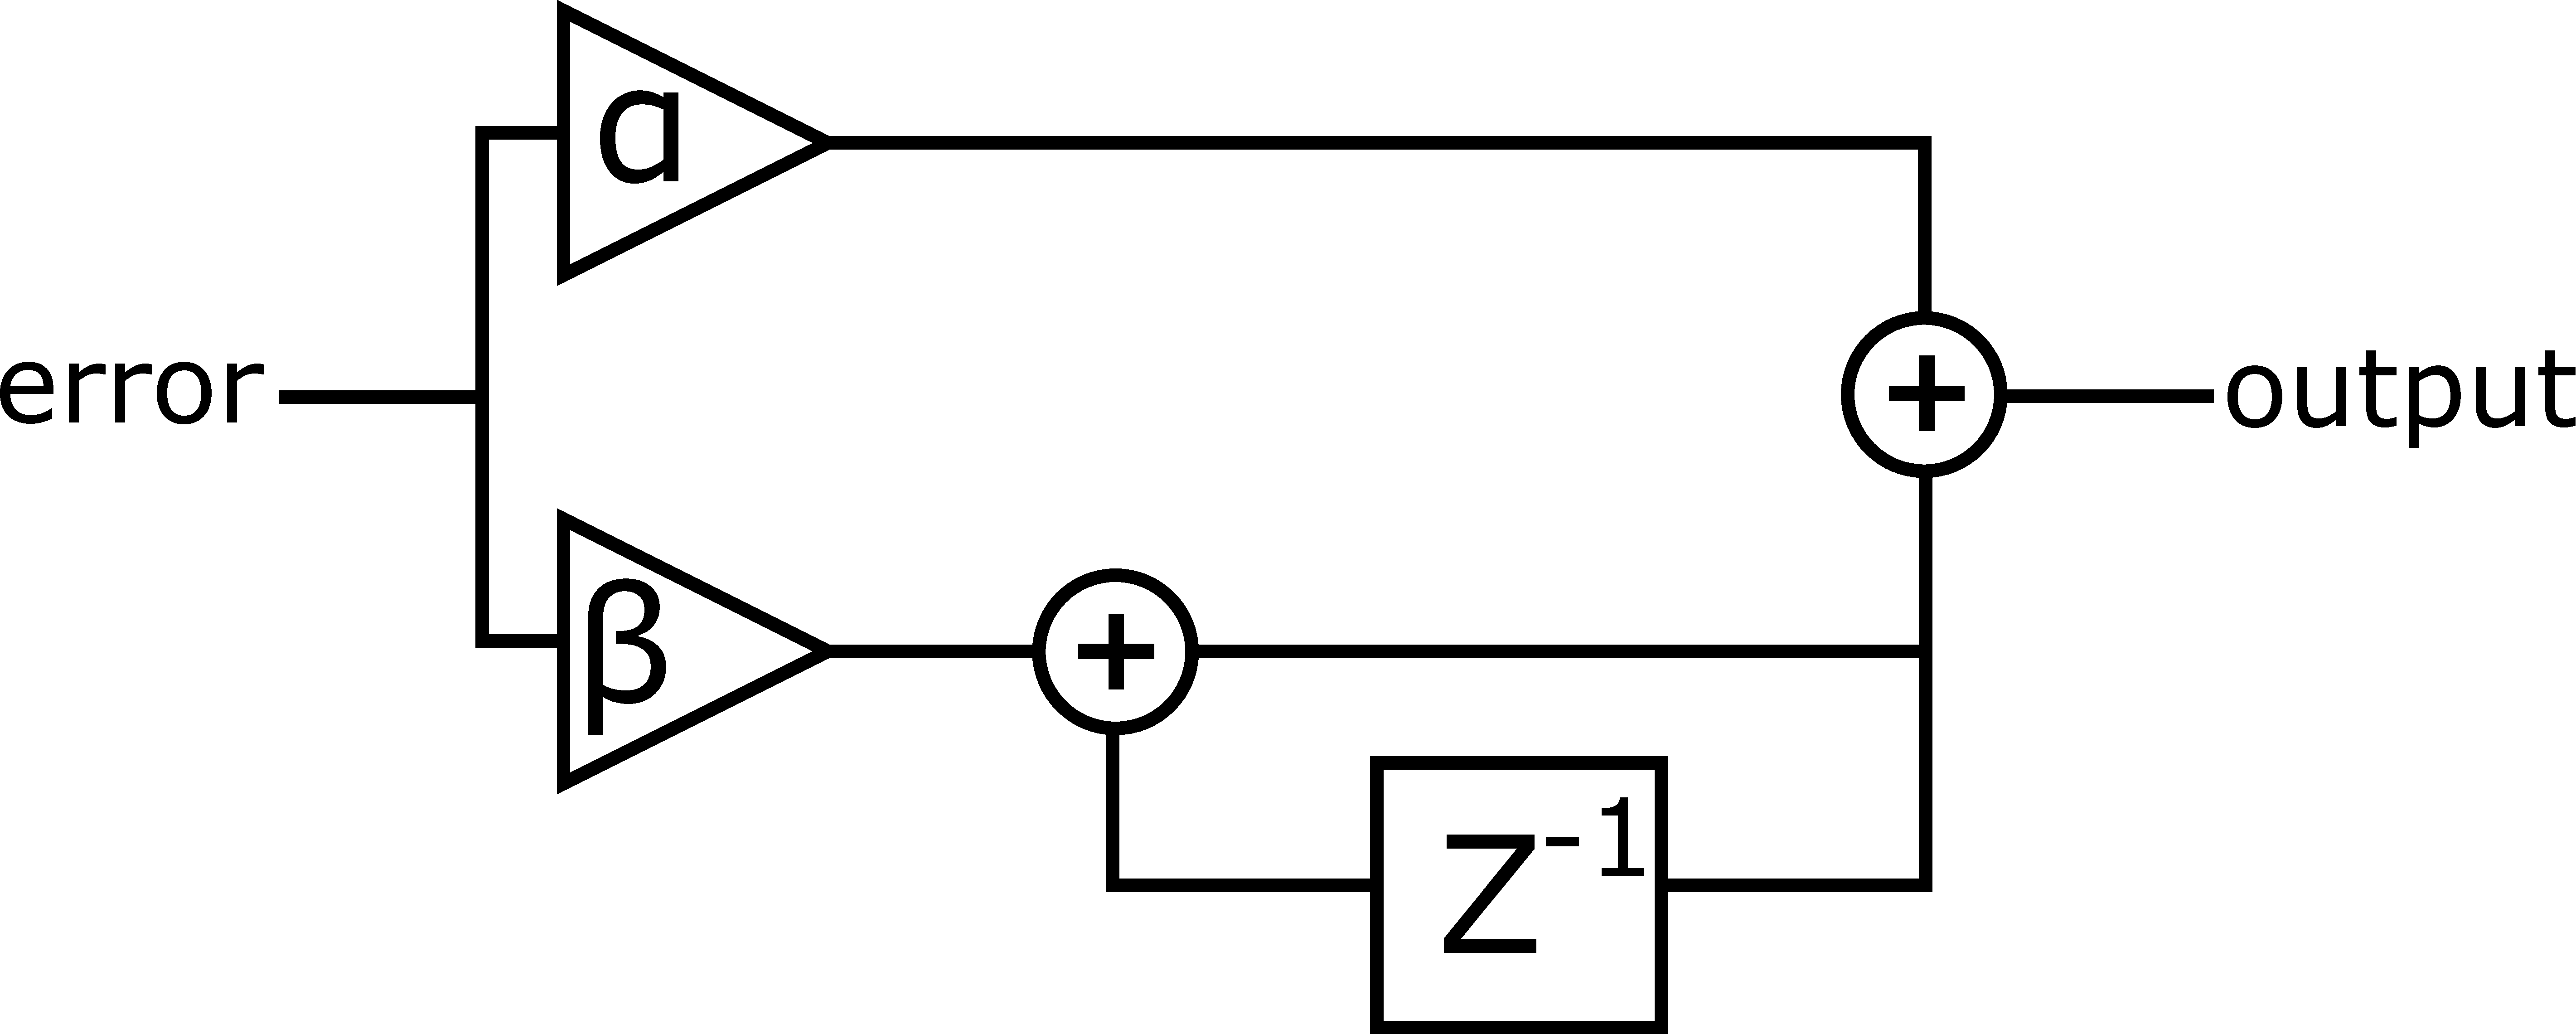
\includegraphics[width=0.6\textwidth]{../simple_pi.pdf}
	\caption[Basic \acs{IIR} \acs{PI} loop filter]{Basic \acs{IIR} \acs{PI} loop filter.}
	\label{fig:iir_pi}
\end{figure}

Again, both integer and fixed-point methods of \ac{LF} design are possible, with the integer method requiring the logic combining the two paths to preserve the relationship between the proportional and integral gains. From the work of Koskin \textit{et al} this known to be several binary orders of magnitude \cite{koskin2018generation}. Failure to preserve a relationship of this order may lead to the \ac{ADPLL} becoming unstable, as in the upper-left region of Figure \ref{fig:gain_grid}. In the fixed-point system the relationship between \ac{kp} and \ac{ki} is preserved during the combination of proportional and integral paths, as both values are aligned using their radix point, before addition is carried out.
\begin{figure}[h]
	\centering
	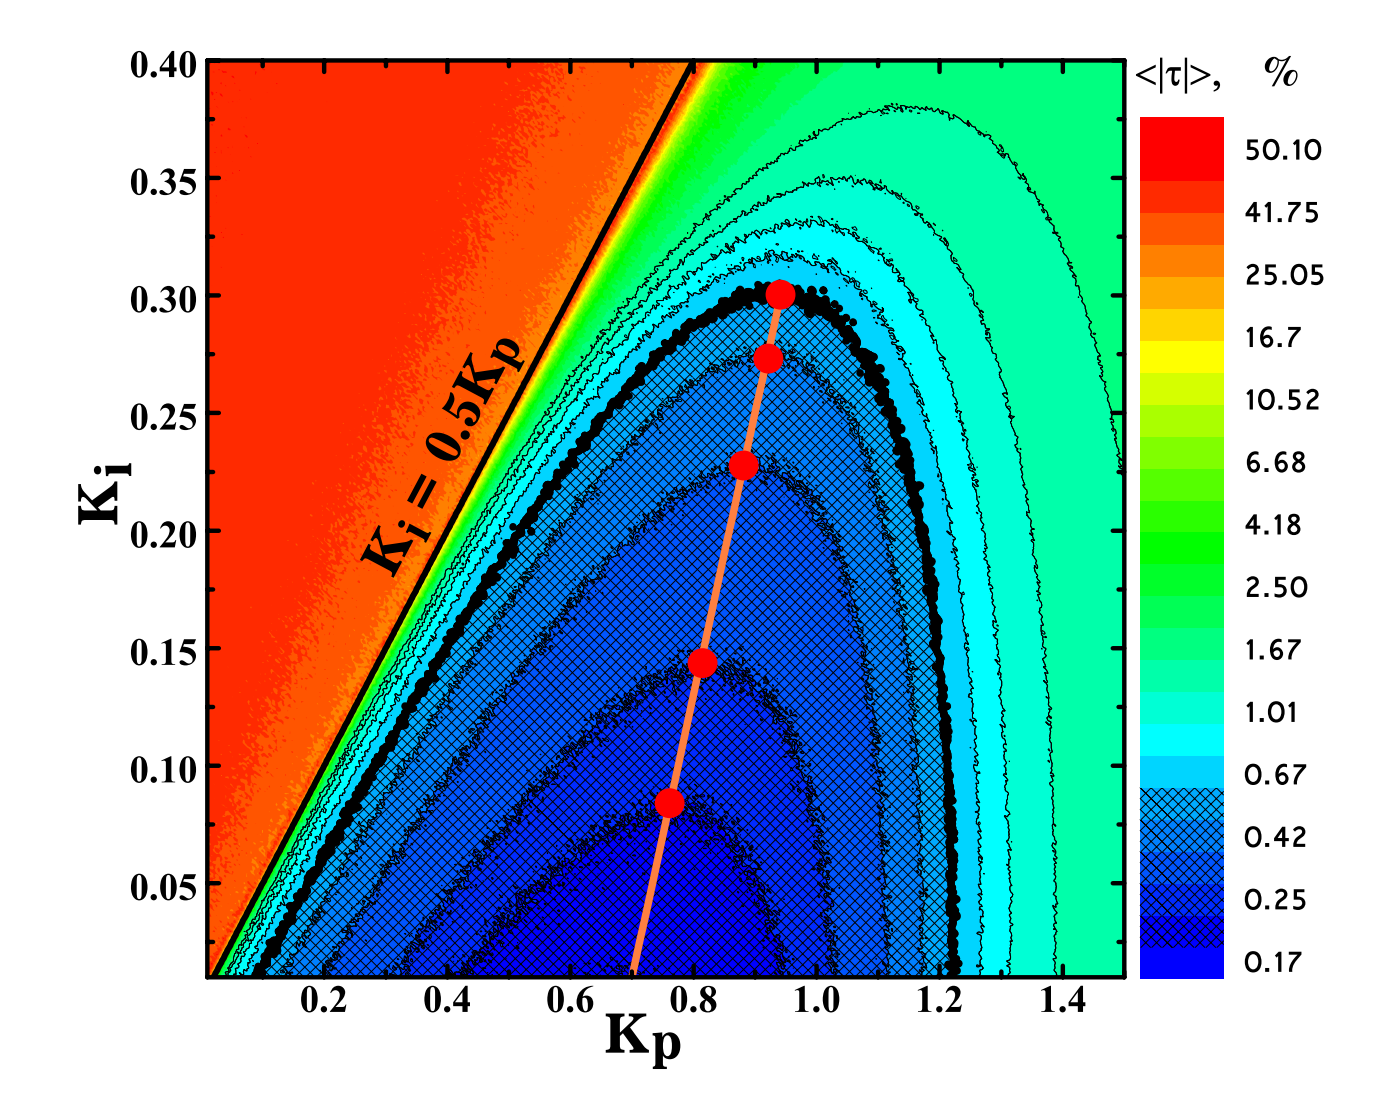
\includegraphics[width=0.6\textwidth]{../eugene}
	\caption[Stability of \acl{LF} gains]{Stability of \acl{LF} gains \cite{koskin2018generation}.}
	\label{fig:gain_grid}
\end{figure}